\documentclass{article}

\usepackage{amsmath}
\usepackage{amssymb}
\usepackage{graphicx}
\usepackage{float}
\usepackage{epstopdf}
\usepackage{hyperref}
\hypersetup {
	urlcolor=blue
}
\graphicspath{./}

\title{Finding Circles In Images With Least Squares Circle Fitting}
\author{Bennet Montgomery 20074049}
\date{2019-03-28}

\begin{document}
	\maketitle
	
	\section*{Abstract}
	This experiment was conducted in order to determine if the presence of circles in an image could reliably be detected by constructing circles of least squares fitting to boundary data of objects in the image. Two images, one containing disks and the other containing office supplies, were processed and circles were constructed to be as close as possible to the perimeters of objects in these images. The root mean standard error of the perimeters of these circles to the actual perimeters of objects in the image were measured with the expectation that least squares circles constructed for circular objects would have lower perimeter errors than for non-circular objects. Ultimately, the least squares fitting circles had low errors of perimeter for circular objects and high errors of perimeter for non-circular objects, proving the effectiveness of this method. 
	\section*{Introduction}
	The objective of this experiment was to determine the effectiveness of using least squares circle fitting via QR decomposition for the task of finding circles in an image based on perimeter data of objects in the image. A common problem in image processing is determining whether or not an image contains circular objects.$^{[1]}$ Least squares circle fitting provides a potential solution to this problem. The relationship between a point $\vec{x}$ on an objects perimeter, the center of the object $\vec{g}$, and the distance from the point to the center $\sigma$ is given by the linear equation:
	 \begin{align}
	 	\left[\begin{matrix}
	 		-2\vec{x}^T & 1
	 	\end{matrix}\right]\left[\begin{matrix}
	 		\vec{g}\\
	 		\sigma
	 	\end{matrix}\right] &= -\vec{x}^T\vec{x}
	\intertext{With the equation above for each point on the perimeter forming an overdetermined linear equation}
		A\left[\begin{matrix}
	 		\hat{g}\\
	 		\hat{\sigma}
	 	\end{matrix}\right] &= \vec{b}
	 \end{align}
	 Which can be solved easily with an economic QR decomposition of $A$ to find the center of the object $\hat{g}$ and the radius of a least squares circle centered on the object $\hat{\sigma}$.$^{[2]}$ We can use this generated least squares circle to determine the circular character of the objected. If the root mean standard error of the residuals between the perimeter points of the generated least squares circle and the perimeter points of the object are much lower than other objects in the image, the object is much more circular than the other objects. If this is an effective method of determining circular character, the disks in the disk image should yield extremely low root mean standard errors, i.e. less than 1, while the rubber bands in the office supplies image should have lower root mean standard errors than the other objects in the image. 
	\section*{Methods}
	Data files provided by Dr. Ellis containing perimeter data of objects in the disk and office supplies images were loaded into matrices and fed into a function {\fontfamily{qcr}\selectfont circlefit()} that utilized an economic QR decomposition of $A$ in equation (2) and back substitution to determine the center points of each object and the radii of the least squares circles for each of the objects. The root mean standard error of the residual between the least squares circle and the real perimeters of each object was then calculated. Finally, the least squares circles were plotted on the appropriate images.
	\section*{Results}
	Objects object 1 to object 6 represent the disks in {\fontfamily{qcr}\selectfont disksimage.png}. Objects object 7 and object 8 represent the rubber bands in {\fontfamily{qcr}\selectfont pillsetgray.png}. Object object 9 represents the rectangular paper in {\fontfamily{qcr}\selectfont pillsetgray.png}. Object object 10 represents the marker cap in {\fontfamily{qcr}\selectfont pillsetgray.png}. The root mean standard errors of perimeters of the least squares circle for each object were:
	\begin{table}[ht]
		\caption{RMSE by object}
		\centering
		\begin{tabular}{ c | c }
			\hline
			\hline	
			object & RMSE \\
			\hline
			object 1 & 0.1216\\
			object 2 & 0.0788\\
			object 3 & 0.1119\\
			object 4 & 0.0785\\
			object 5 & 0.1216\\
			object 6 & 0.1200\\
			object 7 & 3.8099\\
			object 8 & 3.3738\\
			object 9 & 11.0829\\
			object 10 & 7.6020\\
			\hline
		\end{tabular}
	\end{table}
	\begin{figure}[H]
		\centering
		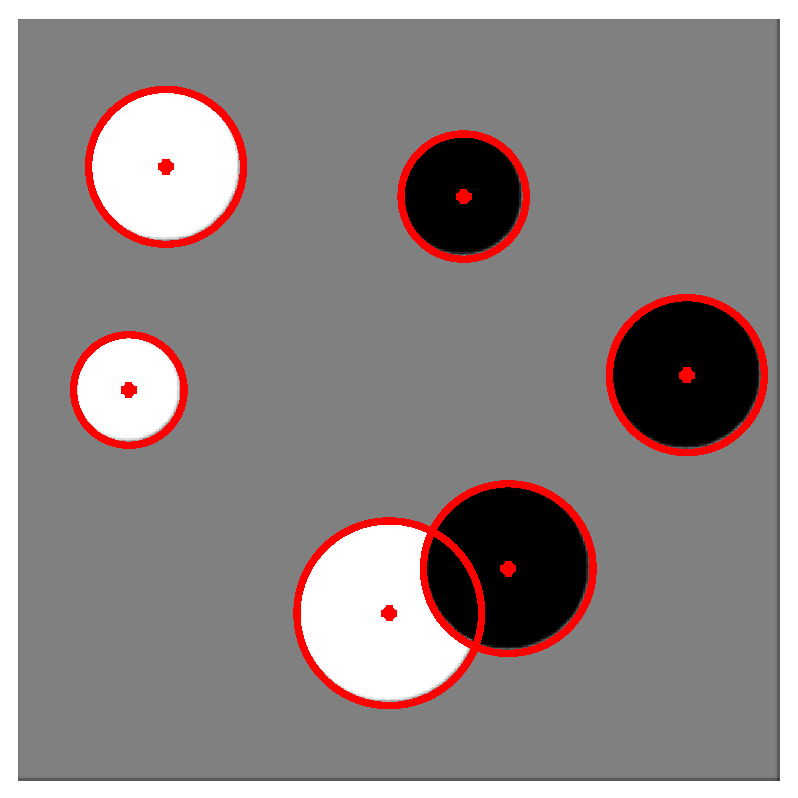
\includegraphics{figure1}
		\caption{The least squares circles of objects 1 through 6 mapped to their associated objects. Notice that the circles almost exactly conform to the perimeters of the disks in this image.}
	\end{figure}
	\begin{figure}[H]
		\centering
		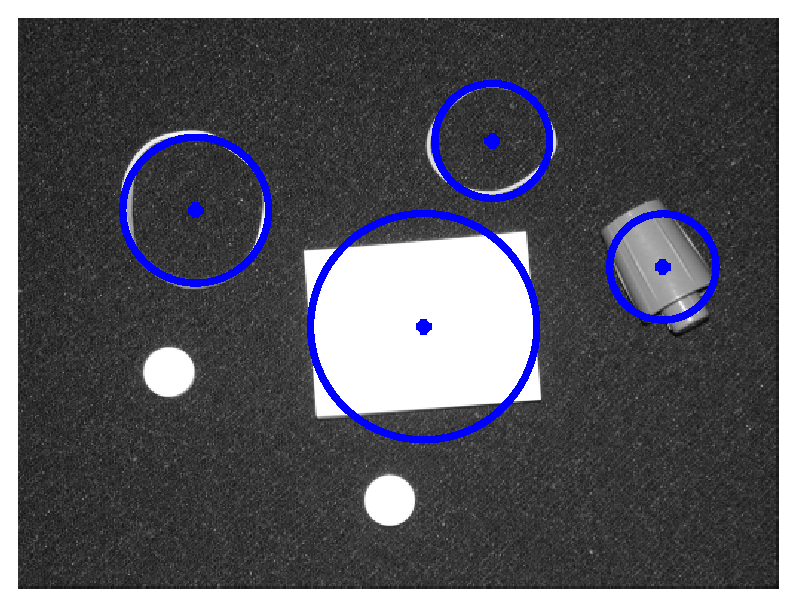
\includegraphics{figure2}
		\caption{The least squares circles of objects 7 through 10 mapped to their associated objects. Notice that the circles do not conform exactly to the perimeters of the office supplies in this image.}
	\end{figure}
	\section*{Discussion}
	The root mean standard errors of perimeters for the least squares circles generated for each of the disks in the disks image were very low, being less than 1 in all cases. The root mean standard errors of perimeters for the least square circles generated for the office supplies was relatively higher, with no circle generated for an office supply having an RMSE lower than 3. The office supplies with the highest circular character, the rubber bands, had by far the lowest RMSEs in the office supplies image with RMSEs of 3.8099 and 3.3738 respectively, implying the least squares circles generated conform much closer with the real perimeters of the rubber bands compared to the paper rectangle (RMSE=11.0829) and the marker cap (RMSE=7.6020). This matches with our expectations, as the disks are extremely circular in character and the rubber bands are the most circular office supplies in the office supplies image. This supports the assertion that the least squares circle fitting method is generally a reliable way of detecting circles in images, as objects with least squares circles with low observed perimeter RMSEs were very likely to be circular in character in this experiment.
	\section*{References}
	1. Ellis, Randy. CISC271, Winter 2019 Assignment \#3 [Internet]. 2019-03 [cited 2019-03-28]. \url{https://onq.queensu.ca/content/enforced/260955-CISC271/Homework/A3.pdf}\\\\
	2. Ellis, Randy. CISC271, Winter 2019 Assignment \#3 Appendix: Least-Squares Circles [Internet]. 2019-03 [cited 2019-03-28]. \url{https://onq.queensu.ca/content/enforced/260955-CISC271/Homework/A3.pdf}
\end{document}